\section{Conexões entre neurônios}
\subsection{Sinapses}
\begin{frame}{Sinapses}
	\begin{columns}[t]
		\column{5cm}
			\begin{figure}[tb]
				\centering
				\caption{Esquema simplificado de uma sinapse química}
				\label{fig:sinapses}
				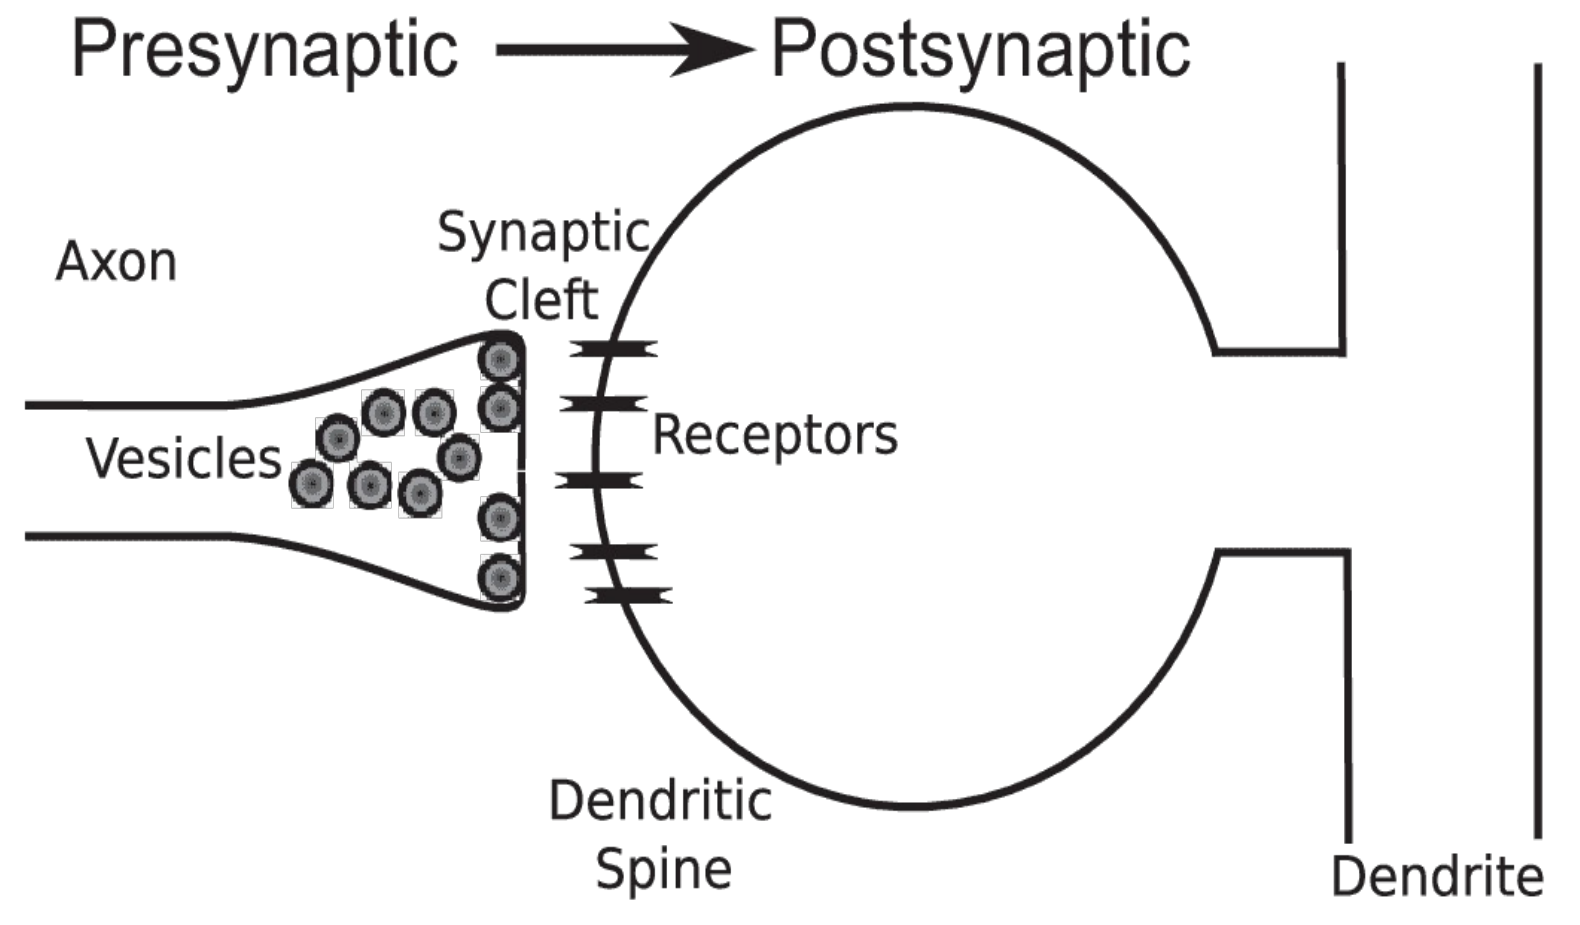
\includegraphics[width=0.9\linewidth]{figs/sinapses}\\
%				\fonte{\cite{miller_introductory_2018}}
				%TODO: trocar figura
			\end{figure}
		\column{5cm}
			\begin{itemize}
				\item Conexão entre dois neurônios;
				\item elétricas: se dão a partir de uma junção entre duas células;
				\item químicas: conectadas por um espaço entre as células por meio de neurotransmissores.
				\item excitatórias: despolarizam a membrana; inibitórias: hiperpolarizam
				\note{glutamato: excita a célula}
				\note{gaba: normalmente inibe}
			\end{itemize}
	\end{columns}
\end{frame}

\begin{frame}{Sinapses}
	\begin{columns}[t]
		\column{5cm}
			\begin{figure}[tb]
				\centering
				\caption{Condutância sináptica em resposta aos potenciais de ação da célula pré-sináptica}
				\label{fig:respostasinaptica}
				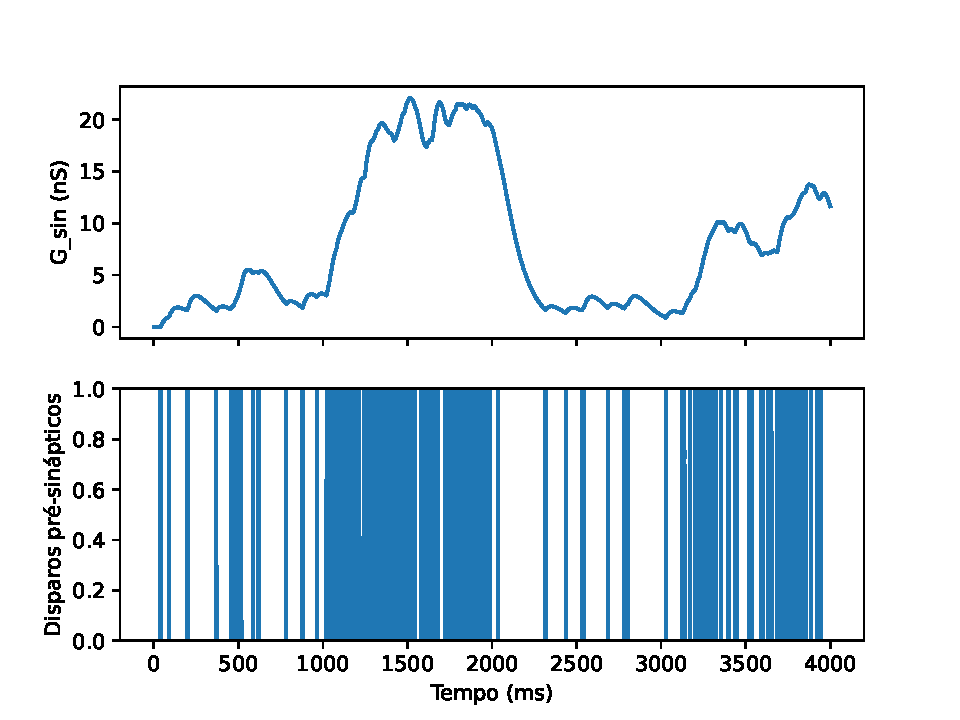
\includegraphics[width=0.9\linewidth]{figs/resposta_sinaptica}
%				\fonte{O autor (\the\year)}
				%TODO: regerar
			\end{figure}
		\column{5cm}
			\[
				\frac{dG_{sin}(t)}{dt}=\frac{-G_{sin}(t)}{\tau_{sin}}
			\]\[
				G_{sin}(t)\mapsto G_{sin}(t)+\Delta G
			\]
			\begin{itemize}
				\item $G_{sin}(t)$: condutância sináptica
				\item $\tau_{sin}$: constante de tempo
				\item $\Delta G$: incremento de condutância
			\end{itemize}
	\end{columns}
\end{frame}

\begin{frame}{Sinapses dinâmicas}
	\begin{columns}[t]
		\column{5cm}
			\begin{figure}[tb]
				\centering
				\caption{Depressão e facilitação sináptica}
				\label{fig:plasticidadecurtaduracao}
				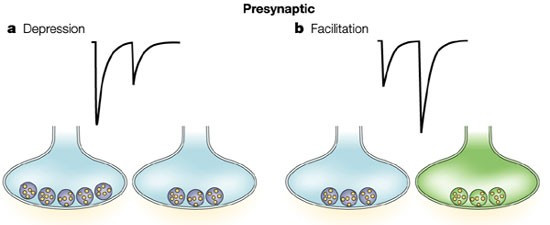
\includegraphics[width=0.9\linewidth]{figs/plasticidade_curta_duracao}
%				\fonte{Adaptado de \cite{blitz_short-term_2004}}
				%TODO: trocar figura
			\end{figure}
		\column{5cm}
			\begin{itemize}
				\item Depressão de curta duração: redução temporária na força sináptica;
				\item Facilitação de curta duração: incremento temporário na força sináptica
			\end{itemize}
	\end{columns}
	\[
		\begin{aligned}
			\frac{dD}{dt}&=\frac{1-D}{\tau_D} &\qquad &D\mapsto D-p_0FD\\
			\frac{dF}{dt}&=\frac{1-F}{\tau_F} &\qquad &F\mapsto F+f_{fat}(F_{max}-F)
		\end{aligned}
		\qquad\qquad \Delta G=G_{max}p_0FD
	\]
\end{frame}

\subsection{Multi-estabilidade}
\begin{frame}{Multi-estabilidade}
	\begin{columns}[t]
		\column{5cm}
			\begin{figure}[tb]
				\centering
				\caption{Comportamento variado do modelo de Hodgkin-Huxley}
				\label{fig:hhdinamico}
				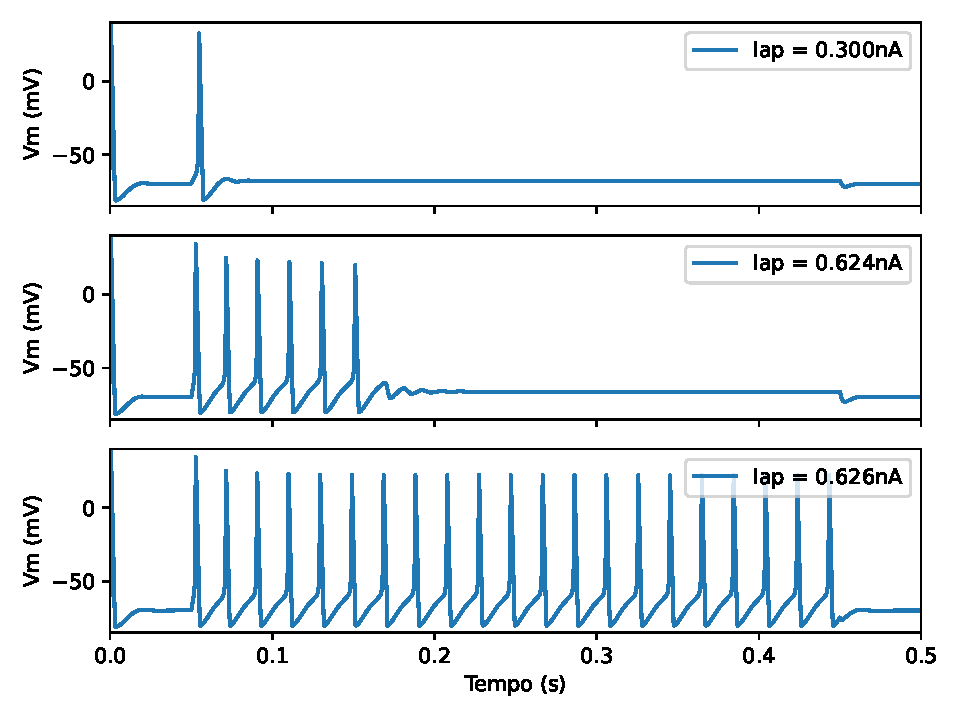
\includegraphics[width=0.9\linewidth]{figs/hh_dinamico}
%				\fonte{O autor (\the\year)}
				%TODO: regerar
			\end{figure}
		\column{5cm}
			\begin{itemize}
				\item Capacidade dos neurônios de manterem múltiplos estados mesmo com a mesma entrada;
				\item Hodgkin-Huxley, por exemplo, pode alternar entre oscilações e ressonância
			\end{itemize}
	\end{columns}
\end{frame}

\begin{frame}{Bi-estabilidade}
	\begin{columns}[t]
		\column{5cm}
			\begin{figure}[tb]
				\centering
				\caption{Cubo de Necker}
				\label{fig:cubonecker}
				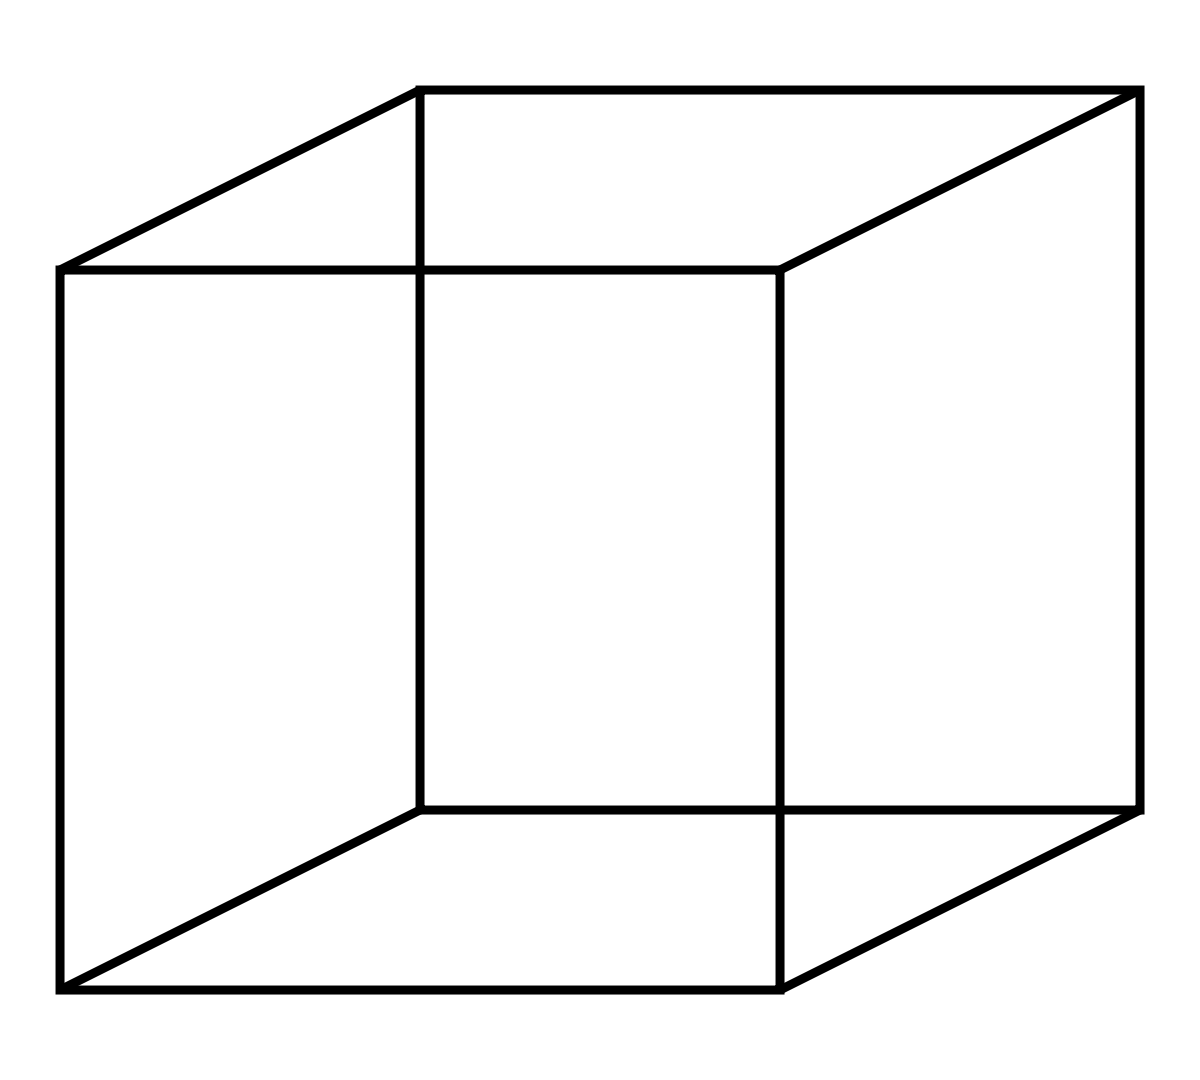
\includegraphics[width=0.7\textwidth]{figs/cubo_necker}
%				\fonte{Domínio público}
			\end{figure}
		\column{5cm}
			\begin{itemize}
				\item Forma mais simples de multi-estabilidade;
				\item dois estados de atividade podem ocorrer;
				\item causa a rivalidade perceptual: estímulos únicos podem ser percebidos de mais de uma maneira
			\end{itemize}
	\end{columns}
\end{frame}


\begin{frame}{Unidades de decisão}
	\begin{columns}[t]
		\column{5cm}
			\begin{figure}[tb]
				\centering
				\caption{Unidades de decisão com feedback recorrente e interconexão}
				\label{fig:unidadesdecisao}
				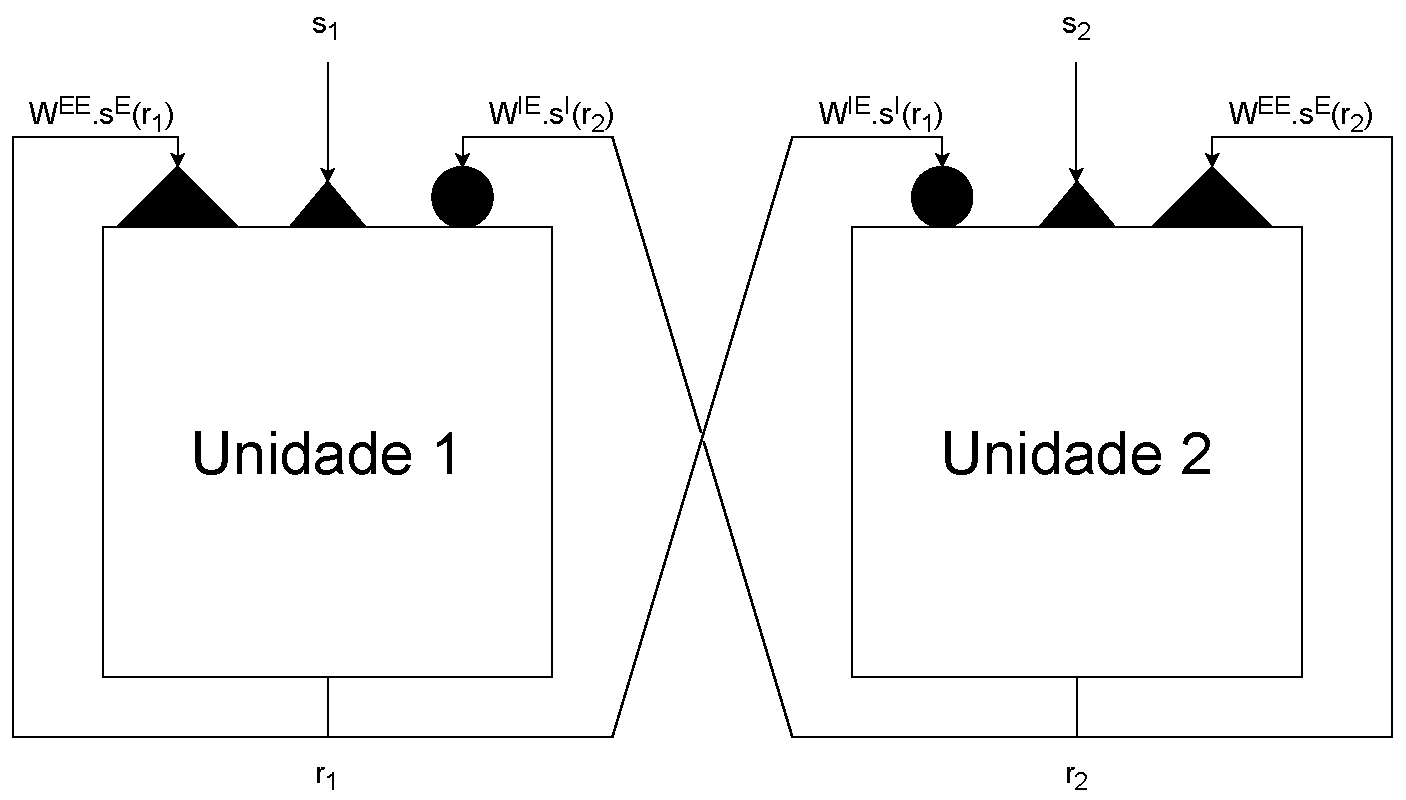
\includegraphics[width=\linewidth]{figs/unidades_decisao}
%				\fonte{O autor (\the\year)}
			\end{figure}
		\column{5cm}
			\begin{itemize}
				\item grupo de neurônios onde é considerada a atividade média deles;
				\note{as entradas diferem por ruído}
				\item unidades podem ter interconexão, com uma inibindo a outra;
				\item podem conectar a si mesmas (\textit{feedback} recorrente).
				\note{o ruído, tanto na entrada quanto dentro da unidade, pode induzir às transições entre estados}
			\end{itemize}
	\end{columns}
\end{frame}

\begin{frame}{Circuito gerador de padrão central}
	\begin{columns}[t]
		\column{5cm}
			\begin{figure}[tb]
				\centering
				\caption{Gerador de padrão central de duas unidades}
				\label{fig:cpg}
				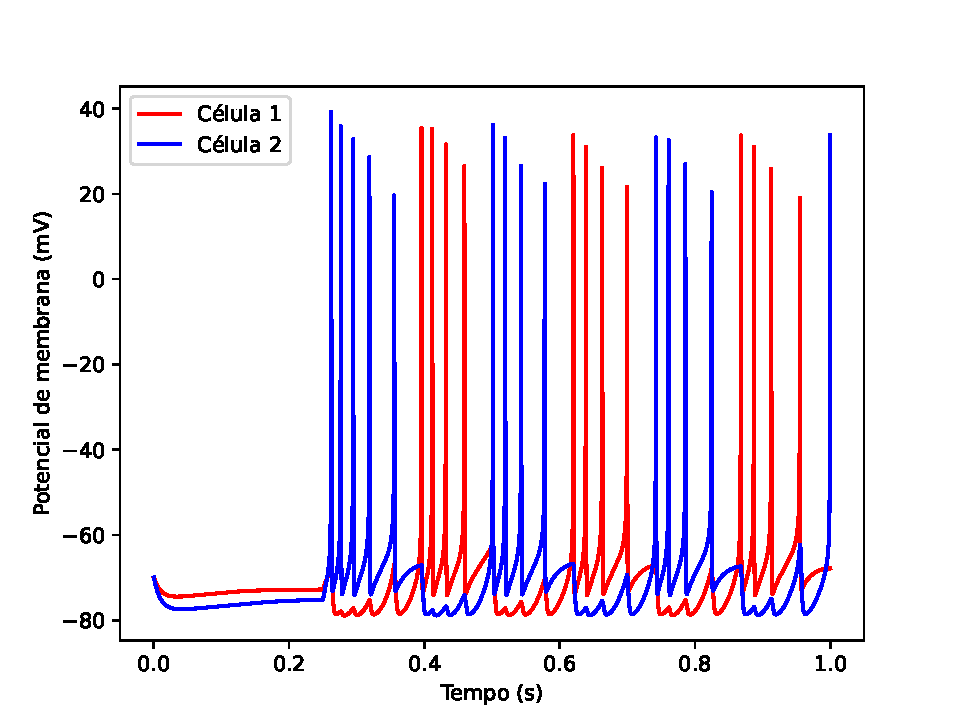
\includegraphics[width=\linewidth]{figs/cpg}
%				\fonte{O autor (\the\year)}
			\end{figure}
		\column{5cm}
			\begin{itemize}
				\item reproduzem padrões rítmicos de atividade neuronal sem receber entradas rítmicas;
				\item a ativação de uma célula inibe a outra;
				\note{correlato com a locomoção: movimento das duas pernas}
				\item muito aplicados em circuitos associados à locomoção de robôs articulados.
			\end{itemize}
	\end{columns}
\end{frame}

\begin{frame}{Circuitos de tomada de decisão}
	\begin{columns}[t]
		\column{5cm}
			\begin{figure}[tb]
				\centering
				\caption{Circuito de tomada de decisão}
				\label{fig:tomadadecisao}
				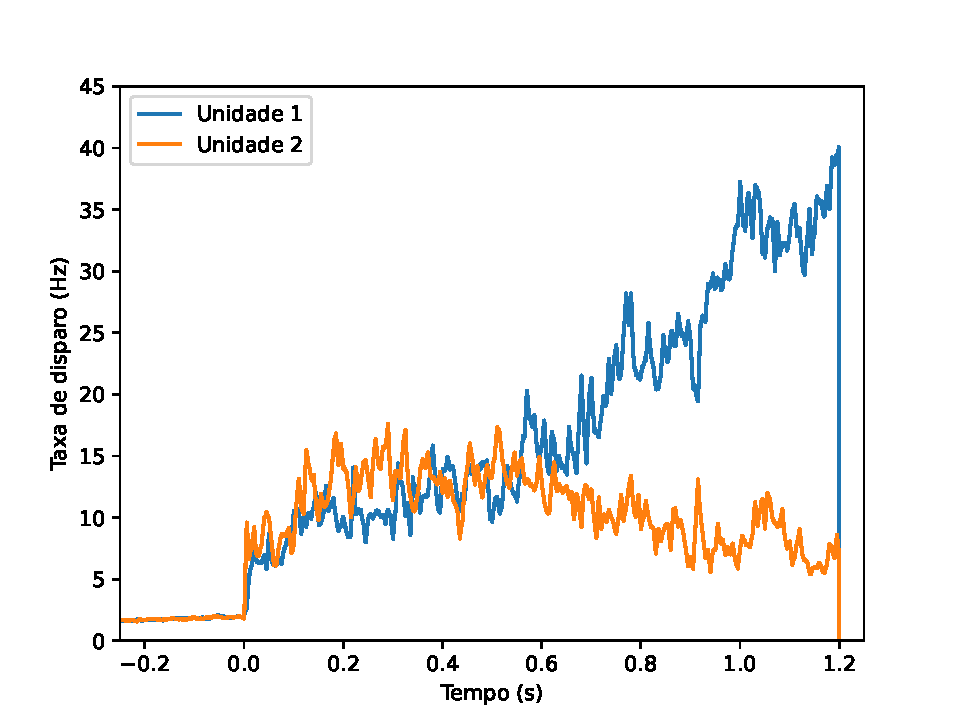
\includegraphics[width=\linewidth]{figs/tomada_decisao}
%				\fonte{O autor (\the\year)}
			\end{figure}
		\column{5cm}
			\begin{itemize}
				\item Acumulam informações sensoriais ao longo do tempo até uma decisão ser tomada;
				\item cada unidade acumula evidências do estímulo ao longo do tempo;
				\item a primeira unidade a atingir um limiar é considerada a vencedora.
				\note{limiar de 40 Hz}
			\end{itemize}
	\end{columns}
\end{frame}

\subsection{Modelos de taxa de disparo}
\begin{frame}{Modelo de Wilson-Cowan}
	\begin{figure}
		\centering
		\caption{Comportamento das simulações do modelo de Wilson-Cowan}
		\label{fig:wilson_cowan}
		\begin{subfigure}[b]{0.3\linewidth}
			\caption{Atividade}
			\label{fig:ww_atividade}
			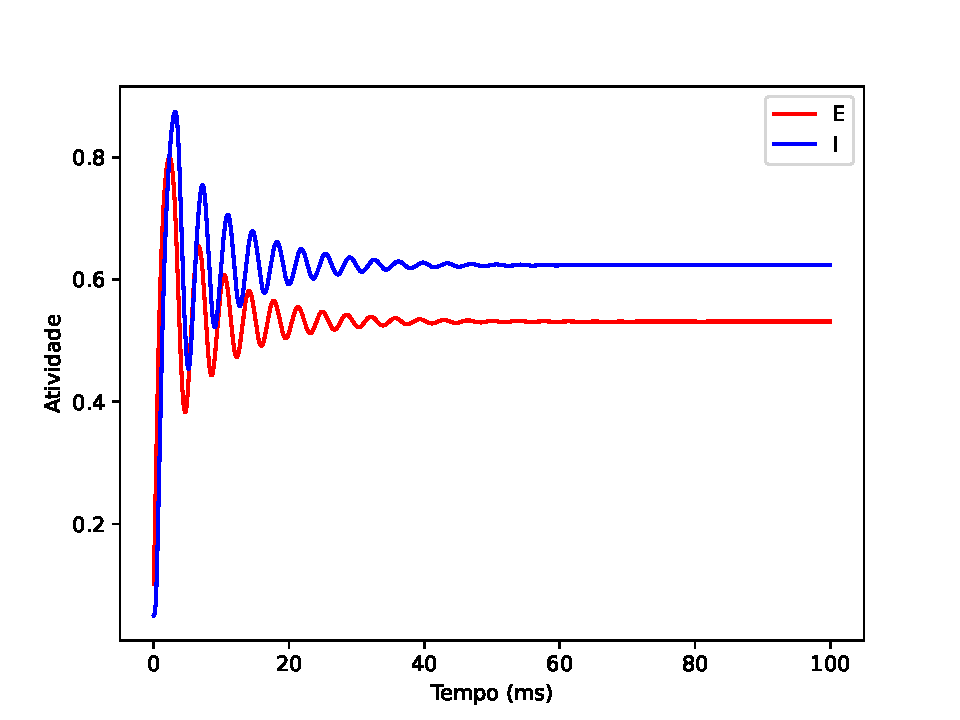
\includegraphics[width=\textwidth]{figs/ww_atividade}
		\end{subfigure}
		~
		\begin{subfigure}[b]{0.3\linewidth}
			\caption{Trajetória}
			\label{fig:ww_trajetoria}
			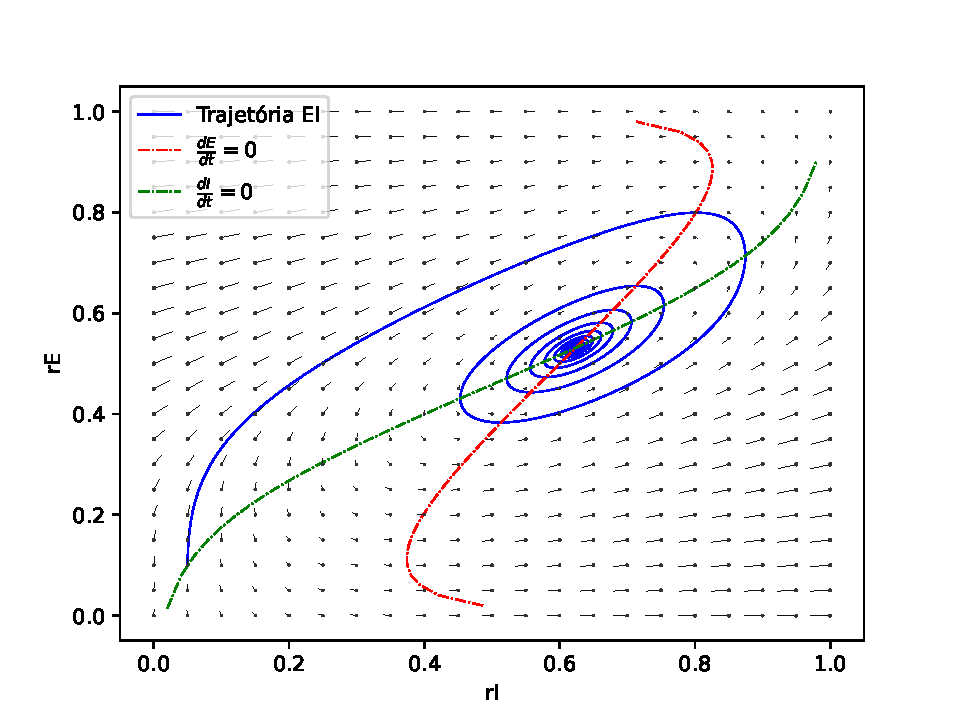
\includegraphics[width=\textwidth]{figs/ww_trajetoria}
		\end{subfigure}
%		\legend{Fonte: o autor (\the\year)}
	\end{figure}
	\[
		\tau_e\frac{\mathrm{d}r_e}{\mathrm{d}t} =-r_e+F_e(w_{ee}r_e-w_{ie}r_i+T_e(t))
		\quad
		\tau_i\frac{\mathrm{d}r_i}{\mathrm{d}t} =-r_i+F_i(w_{ei}r_e-w_{ii}r_i+T_i(t))
	\]
	\note{considera subpopulações excitatórias e inibitórias}
	\note{sistemas dinâmicos: se alteram ao longo do tempo (taxa de disparo)}
	\note{nullcline: trajetória quando as derivadas são nulas (taxa de disparo não se altera)}
\end{frame}

\subsection{Aprendizado e plasticidade de longa duração}
\begin{frame}{Plasticidade de longa duração}
	\begin{columns}[t]
		\column{5cm}
			\begin{figure}[tb]
				\centering
				\caption{Plasticidade dependente do tempo de disparo (STDP)}
				\label{fig:stdp}
				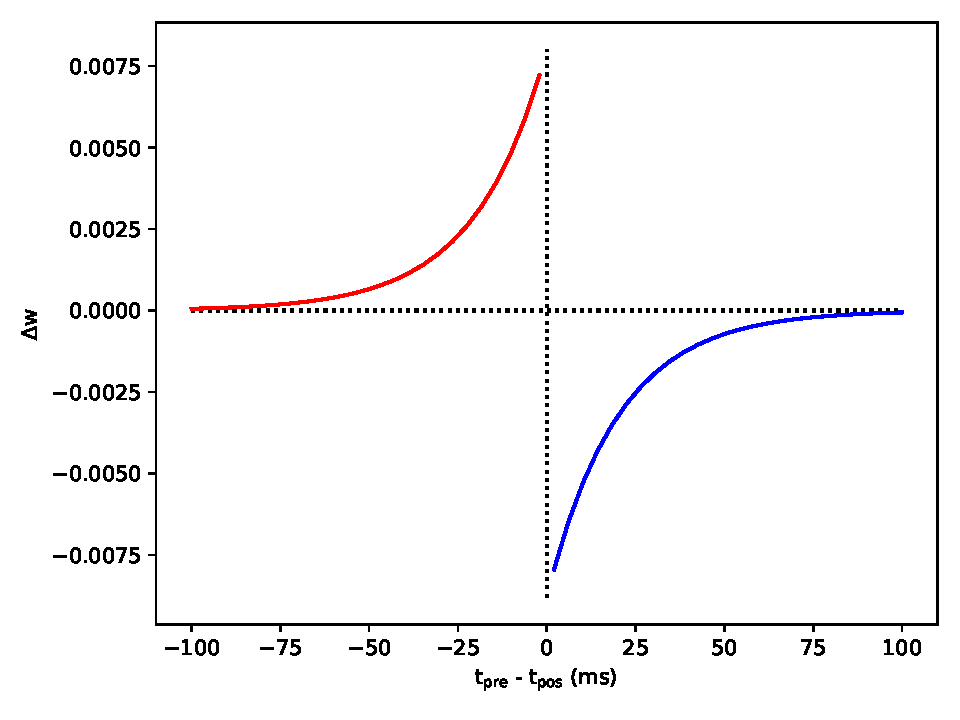
\includegraphics[width=\linewidth]{figs/stdp}
%				\legend{Fonte: o autor (\the\year)}
			\end{figure}
		\column{5cm}
			\begin{itemize}
				\note{Regra de Hebb: se um neurônio A excita um neurônio B repetidas vezes, então a sinapse entre os dois deve ser fortalecida}
				\item potencialização de longa duração: crescimento da força de conexão sináptica;
				\item depressão de longa duração: diminuição da força;
				\[
					\Delta_w=\begin{cases}
						A_+\exp(\Delta t/\tau_+)\text{, }\Delta t<0\\
						-A_-\exp(-\Delta t/\tau_-)\text{, }\Delta t\geq0
					\end{cases}
				\]
				\note{$A_+$ e $A_-$: valores máximos de modificação sináptica}
				\note{$\tau_+$ e $\tau_-$: faixas de intervalo entre disparo das células pré e pós-sinápticas}
			\end{itemize}
	\end{columns}
\end{frame}
